% Copyright (C) 2013 Thomas L. Kula
% All Rights Reserved
%
% See the file LICENSE for license terms.
\documentclass[12pt]{article}
\usepackage{graphicx}
\usepackage{rotating}
\usepackage{fix-cm}
\usepackage{multirow}
\setlength{\paperwidth}{5.5in}
\setlength{\paperheight}{8.5in}
\setlength{\textheight}{7.45in}
\setlength{\topmargin}{-1.0in}
\setlength{\oddsidemargin}{-0.5in}
\setlength{\evensidemargin}{-0.5in}
\setlength{\textwidth}{4.0in}
\setlength{\parindent}{0in}
\setlength{\parskip}{3mm}
\usepackage[print]{booklet} \nofiles
\source{\magstep0}{5.5in}{8.5in}
\target{\magstep0}{11in}{8.5in}
\setpdftargetpages
\pagestyle{empty}
\begin{document}


\begin{center}
{\fontsize{36}{48}\selectfont \textsc{Haiku a Day }}
\end{center}

\vspace*{3.5cm}

{\fontsize{20}{40}\selectfont 

A siren's sweet call

Bright and jangly down the street

Get your ice cream here


}

\vspace*{5.0cm}
\begin{center}
{\large{Issue 94: April 2013}} \\[5mm]
{\fontsize{8}{8}\selectfont  \textsc{ St. Joshua Norton Press }} \\[1mm]
{\fontsize{6}{6}\selectfont Mathom House by the Cloisters \textbar The People's Republic of Ames }
\end{center}


\newpage

There comes a time when a man's thoughts turn to grilling. That time is now.

--- Thomas

http://kula.tproa.net/had/ \\
kula@tproa.net

Download this and previous HADs at the website, so you can
print out your own (DIY, yeah!) or if you want me to send
you one, send me your address, and maybe a stamp if you
are feeling nice. Or send me something you've made ---
trades always appreciated, postcards are nice too.

\vfill

1 April 2013

Stupid --- stupider: \\
Lame April Fools jokes anguish. \\
Put thought into it

2 April 2013

Tour the dark side \\
Discover that they have cake \\
To hell with goodness

\newpage

3 April 2013

Foam lapping the shore \\
A gurgling river flows by \\
Cares washing away

4 April 2013

Don't want a monkey \\
Unless it's a smart monkey \\
One that will wear pants

5 April 2013

In a man's life, there  \\
Comes a time for seersucker \\
For this man, today

6 April 2013

A saucer, a cup \\
Hot water becoming tea \\
Morning in Inwood

7 April 2013

In the cracks of cheese \\
Tasty mold making it bleu \\
A dressing awaits

8 April 2013

A bird in flight turns \\
Into the sun, and too close \\
Finds infinity

9 April 2013

Filing files \\
F for file, R for rasp \\
This work grinds away

\newpage

10 April 2013

AE-35 \\
Sending a lonely signal \\
A whisper, a fault

11 April 2013

Constant consonant \\
The base of words, not flashy \\
Not sharp like vowels

12 April 2013

A cherry purches \\
Proud like a queen on a cloud \\
An ice cream soda

13 April 2013

A doctrine I have: \\
An elephant on a crane \\
Is not stood under

14 April 2013

Morning energy \\
Quickly turns to lazyness \\
Do things tomorrow

15 April 2013

A roll of string falls \\
Grasping at it makes it worse \\
I grab, it races

16 April 2013

A tiny gate on \\
A tiny patch of front lawn \\
A tiny dog sits

\newpage

17 April 2013

What a shame it is \\
To be a fire fighter \\
Fire trucks boring

18 April 2013

``They're the wrong trousers,'' \\
he said, with his hands shaking, \\
``And they have gone wrong!''

19 April 2013

Old British guys in \\
Academic dress, nerding \\
Out all day today

20 April 2013

A good thing better: \\
A cute guy riding the bus \\
Reading {\em Good Omens}

21 April 2013

Apartment contrasts: \\
Some things done very cheaply \\
Some places marble

22 April 2013

Pocket watch unwatch \\
The shell exists but no time \\
No time right or wrong

23 April 2013

Retire early \\
Too much Chinese food, and zines \\
Then I fall to sleep

\newpage

24 April 2013

Flywheels spinning up \\
A low hum becomes a whine \\
Ready to burst forth

25 April 2013

Ephemeral song \\
By an orchestra not there \\
Makes me march in time

26 April 2013

The day done, gladness \\
That all of the days are done \\
At least for two days

27 April 2013

First there are pickles \\
Biscuits and vegan gravy \\
Too much food to eat

28 April 2013

Clouds stretch for miles \\
Bursting with light, the sun sets \\
The clouds float away

29 April 2013

Must learn the organ \\
Want to play Animals songs \\
Intentions are good

30 April 2013

Tape not sticking well \\
Package keeps unraveling \\
Break out the good stuff


\newpage

\begin{center}
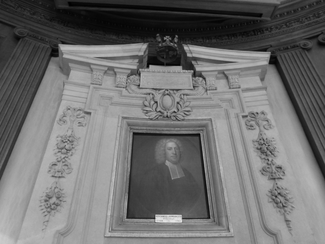
\includegraphics[width=325pt]{burgon.png}
The Reverend Samuel Johnson, S.T.D \\
President of King's College 1754 - 1763 \\
(S.T.D. meaning something very different back then)\\
19 April 2013 \\
{\tt kula.tproa.net/photos/2013/20130419-burgon}
\end{center}

\newpage

\thispagestyle{empty}
\vspace*{12cm}
\begin{sideways}
\Large{St. Joshua Norton Press}
\end{sideways}
\begin{sideways}
\Large{PO Box 250138}
\end{sideways}
\begin{sideways}
\Large{New York NY 10025}
\end{sideways}


\end{document}


